\chapter{Výroba růže}
Původním záměrem bylo vytvořit svítící lampičku ve tvaru růže. Vzorem pro výrobu růže byl plastový uzávěr od lahvičky s vůní ve tvaru růže, s rozměry: přibližně 6~cm široký a 3~cm vysoký. Tato růže byla použita na výrobu formy. Forma byla později opakovaně použita na výrobu tří téměř identických odlitků.
%Mohla jsem se domluvit s umělcem, aby růže byla ze skla, mohla jsem ji vytisknout na 3D tiskárně. Já jsem se ji ale rozhodla odlít, protože mě zaujala práce s křišťálovou pryskyřicí. 

%*Obrázek k vzoru*


\section{Silikonová forma}

Rozhodla jsem se že formu vyrobím z odlévacího silikonu. Odlévací silikony mají skvělé kopírovací vlastnosti a mají i dostatečnou pružnost, potřebnou k dobrému odformování komplikovaných výrobků. Pokud je forma dobře udělaná, lze ji používat opakovaně.



\begin{figure}[htbp]
	\centering
%	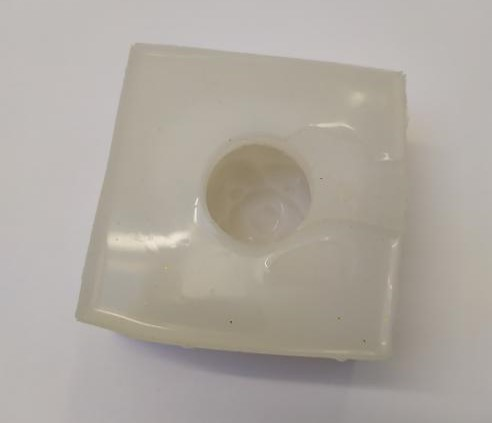
\includegraphics[width=1\textwidth]{img/05odl/Siliconemold.jpg}
%	\caption{Silikonová forma}
	%	\label{fig:install-sdk-3}
\end{figure}
 

%\subsection{Leukopren žlutý silikon}

\subsection*{Adiční silikon GMS A30 (Silikon)}

%Druhým druhem silikonu byl Adiční silikon GMS A30.
Na výrobu formy jsem použila \textit{Adiční silikon GMS A30}  \cite{silikon} z internetového obchodu \textit{Levnetmely.cz}  \cite{tmely}. Jedná se o dvousložkový, dobře tekutý silikon s velmi dobrou kopírovací schopností, schopný zkopírovat jak povrch obyčejného papíru, tak dřeva s letokruhy.

Tento silikon se používá na výrobu forem, například pro odlévání epoxidové pryskyřice, sádry nebo vosku. Dále se využívá na výrobu těsnění nebo zalévání součástek v elektroprůmyslu.


\subsection*{Práce se silikonem}
Balení \textit{Adičního silikonu GMS A30} se skládá ze dvou složek: složky~A a složky~B. Tyto dvě složky se musí smíchat v hmotnostním poměru 1:1. Při míchání je potřeba dát pozor, aby se do silikonu nedostaly bublinky, které by mohly znehodnotit formu a zdeformovat kopírovaný tvar.

V případě použití kompresoru by stačilo veškerý vzduch odsát, a tím způsobem se zbavit bublinek. Protože ale kompresor nevlastním, malému množství bublinek jsem se nevyhnula. Při práci se silikonem je potřeba dbát na bezpečnost práce a při manipulaci se silikonem mít na sobě ochranné brýle a rukavice.

%*Obrázek formy*

Po přibližně 24 hodinách bývá výsledkem středně tvrdá, odolná silikonová pryžová forma, se skvělým odformováním. V našem případě ale odformování problematizoval komplikovaný tvar květiny.


\begin{figure}[htbp]
	\centering
	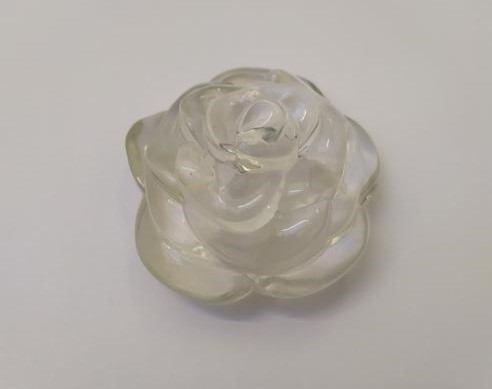
\includegraphics[width=0.5
	\textwidth]{img/05odl/Rose.jpg}
	\caption{Odlitá růže}
	%	\label{fig:install-sdk-3}
\end{figure}

\section{Pryskyřice}
Křišťálová pryskyřice  \cite{pryskyrice} (Epoxy Resin) je dvousložková průhledná odlévací směs často používaná na výrobu bižuterie, různých dekorací nebo glazování povrchů. Dobře se s ní pracuje, její zápach je nízký, a po vytvrdnutí je její povrch lesklý a nesmršťuje se. 

Pro realizaci tohoto projektu byla pryskyřice vybrána z důvodu dobré imitace skla a~zároveň nízké křehkosti tohoto materiálu. 
%Tato pryskyřice byla vybrána i z důvodu, že dobře imituje sklo, ale zase postrádá jeho křehkost.
Při odlévání růže byla konkrétně použita křišťálová pryskyřice od firmy \textit{Pebeo}  \cite{pebeo}, sehnatelná v jakémkoliv specializovaném uměleckém obchodě nebo obchodě pro kutily. 


\subsection*{Práce s pryskyřicí}

Pro použití pryskyřice je třeba smíchat složku A a složku B. Tyto dvě složky se  smíchají v~hmotnostním poměru 2:1. Při odvažování je důležitá přesnost. Dále je duležité obě složky dobře promíchat, jinak by mohlo dojít ke špatnému vytvrzení výrobku. Při míchání je třeba dávat pozor, aby se do pryskyřice nedostaly bublinky. Poté se daná směs vylije do předem připravené formy nebo na povrch, který chceme glazovat. Pryskyřici trvá 24 až 48 hodin, než zatvrdne. Křišťálová pryskyřice je chemikálie a proto se, z důvodů možných alergických reakcí a podráždění dýchacích cest, doporučuje při manipulaci s pryskyřicí nosit ochranné brýle, rukavice a respirátor. 

Před vylitím pryskyřice do předem připravené formy je prý vhodné danou formu vytřít speciální vazelínou, která prodlužuje životnost formy a která brání jejímu poškození při vyjímání odlitku. Tento způsob se ale v našem případě, při odlévání pryskyřičné růže, neosvědčil. Vazelína se smíchala s odlévací pryskyřicí a ve výrobku se vytvořil bílý mléčný kal, který znehodnotil výrobek a pokazil sklovitý dojem pryskyřice.







